%************************************************
\chapter{Introduction}\label{ch:introduction}
%************************************************
%\section{Introduction} \label{intro:intro}


\section{Biologically-Inspired Soft Robotics}

Softness and compliance are two notable features that make humans
and animals capable of interacting efficiently in a complex environment.
Thus, in the field of robotics, understanding biological processes
and systems have always been a great source of inspiration for engineers
to develop more capable robots. Even though traditional robots
are well-read and investigated, they are as yet unable to adequately
fulfill the requirements of the interactions needed in variable and
unpredictable working states.

Although the capabilities of the traditional-bodied robots have seen
a lot of significant development, the demand for studying various
biological processes and developing systems which are capable of
soft and continuous interaction with the environment has led many
researchers to open the gateway of a new field of research known as
the soft robotics \citep{rus2015}. In the previous couple of years, the area of soft
robotics has progressed toward becoming a very much characterized
discipline with working practices.

Soft robotics is an area where the robots are designed by using soft
and compliant modules. The advantage of soft robots over rigid body
counterparts are involving infinite degrees of freedom and different
movements \citep{Yap2016}. Robots which can completely mimic various biological
process can be developed by combining multiple functional units
strategically to act as a single unit, which generates smooth actions
and adaptability to different environmental conditions. Some of the
advantages of soft robots are continuous body motion, large-scale
deformation, safe human-robot cooperation, minimal effort production
\citep{Katzschmann2016,Argiolas2016}, and basic manufacture with negligible coordination \citep{Argiolas2016}.

In rigid body control, the locomotion of which can be described by
six degrees of freedom but in soft-bodied robots, the movement cannot
be limited to planar motions. Due to the bending, buckling, wrinkling,
stretching, twisting, compressing, etc. nature of the soft materials,
developing a control system for such robots are very challenging. Controlling
soft robots demand new lines of modelling, control, dynamics
and advanced level planning \citep{rus2015}. One of the important aspects of
controlling bio-inspired soft robots is that all the parts of the robot
continuously interact and inspire each other. Despite the fact that a particular accord on these principles is developing in the soft robotics and
its related societies, the young field of bio-inspired soft robotics still
wants a robust and steady base like control theory for rigid robotics \citep{Pfeifer2007}. The theory needs to be further developed, and a substantial amount
of work toward a better understanding of how the behaviour of the
robot is influenced by its underlying governing dynamics rather than
controlled is still needed to be achieved \citep{Pfeifer2012}. To have a grasp of the
science, researchers are performing an exhaustive number of different
experiments on the soft robots which result in the collection of
extensive experimental data.

\section{Machine Learning Modelling and Control in Soft Robotics}

\ac{ML} as an arrangement of strategies that can naturally
distinguish patterns in data, and afterwards utilise the revealed
patterns to foresee future data or to perform different sorts of decision
making under vulnerability. Use of \ac{ML} strategies to
massive databases is called as data mining \citep{Alpaydin2020}. However, it should be
noted that even when one has an evidently large dataset, the effective
number of data points for particular cases of interest might be quite
small. In fact, data from a variety of spaces shows a property known
as the long tail, which implies that a couple of things are exceptionally
similar. However, most things are very uncommon. For instance,
twenty percent of Google hunts every day have never been seen \citep{Murphy2012}.
This implies the centre measurable issues concerning generalising
from small examples sizes, are still exceptionally pertinent even in the
era of big data.

\section{Biological Swallowing and Endoprosthetic Stenting}

Swallowing is a complex but orderly physiological process transporting
saliva or food from the mouth to the stomach, aided by peristaltic
contractions of the esophageal wall, generated by \ac{CPG} \citep{Jean2001}. Any esophageal impairment compromises the
efficiency of swallowing, is known as dysphagia. Severe pathologies,
for instance, benign esophageal strictures from various injuries,
\ac{EC}, and esophageal perforations, distressing lumen patency
explicitly leading to dysphagia \citep{Garcia2010}. Unaccompanied by
comprehensive care, a vicious cycle materializes as malnutrition and
dehydration aggravating the dysphagia itself, subsequently increasing
morbidity and even mortality.

A silicone covered \ac{SEMS} is a tubular
braided mesh of interwoven helical springs made of corrosionresistant
materials, like nitinol, stainless steel, and polymers. Malignant
and benign esophageal strictures from \ac{EC}, can be
addressed with the endoprosthetic stent placement, commonly known
as esophageal stenting \citep{hanawa2009materials}. These stents are proven to be efficient endoprosthetic
management for both malignant and benign esophageal
strictures, as they could hold open the esophagus and hence, relieve
the impediments of compromised lumen patency in such cases \citep{hirdes2013vitro}.

However, this method of palliative treatment does have its inadequacies,
and one of the significant shortcomings is stent migration,
which is the movement of the implanted stent from its initial position,
caused due to the stent interaction with the continuous peristaltic
contractile forces of the esophageal wall \citep{sharma2010role}. Stent radial force (RF), force applied by the stent on the esophageal lumen, is a crucial design parameter of a stent for maintaining the in situ lumen patency, which is, unfortunately, still an unknown parameter due to the poorly understood association of the RF and clinical outcomes. The efforts to mitigate
migration, to improve stent removability and flexibility, and to ensure
stent patency have revolutionized the stent designs. To study stent
inadequacies for improving stent design, conventional techniques like
manometry and videofluoroscopy on the patients are less preferred
because the techniques are not very comforting for the patients, and
there are major ethical concerns associated with such kind of studies.
Thus, evidence to show which stent design is better than the other is
confined to a few \ac{RCT} in patients with
malignant esophageal strictures \citep{hirdes2013vitro}.

\section{Robotic Soft Esophagus}

The current research is an augmentation of a research program that
explores biomimetic esophageal swallowing. A \ac{RoSE} has been developed as an alternative platform for mimicking
the human swallowing process under different rheological and
medical conditions (\autoref{fig1_RoSE_f1}) \cite{Dirven2014}. The capability of \ac{RoSE} is to generate
peristaltic waves of different characteristics similar to the waves
generated when food bolus travels from upper to the lower esophagus
in humans.

\begin{figure}[bth]
	\myfloatalign
	{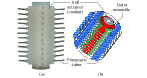
\includegraphics[width=\linewidth]{images/Ch1/fig1_RoSE_f1}} \quad
	\caption[Robotic Soft Esophagus (RoSE)]{Robotic Soft Esophagus (RoSE). (a) RoSE actuator (conduit), and (b) isometric view of \ac{CAD} assembly of RoSE.}\label{fig1_RoSE_f1}
\end{figure}

\ac{RoSE} is made up of Ecoflex 00-30 (Smooth-On, USA), which is a soft
and highly stretchable platinum-catalyzed silicon rubber. The physical
dimension of \ac{RoSE} matches the attributes of the human esophagus
\cite{Dirven2014}. \ac{RoSE} has twelve equally spaced layers, and in each layer, four
pneumatic chambers are present surrounding the conduit. The purpose
of these air chambers is to deform sequentially layer by layer
under the supplied air pressure in such a way that the shape of the
deformation can take the form of a traveling peristaltic wave from
the top layer to the bottom layer \cite{Dirven2015}. \ac{RoSE} is a true example of a
robot mimicking a biological process, and performing tests on such a
robot instead of a human being can save the researchers from ethical
concerns and accessibility time, and it can widen the range of different
measurements and evaluation schemes \cite{Dirven2015}.


\section{Research Motivation}

There are two reserach motivation for this study. The first motivation of
this research is to validate \ac{RoSE} as a novel in vitro platform to perform
a wide-ranging assessment of stent-behavior. The second motivation
of this research is to set out on another convention: establishing and
implementing \ac{ML} techniques as the first and foremost
above traditional analysis.

\subsection{Motivation 1}

Testing bolus formulation and transport, stent behavior assessment,
and swallow efficacy with clinical trials are hindered by the interperson
swallow and the inter-swallow variability in human test subjects.
Besides, due to the less known relationship between the mechanical
properties of the esophageal stents and their clinical outcome, the
stenting guidelines are still poorly defined. Further, evidence from the
\ac{RCT} that can be used to test the clinical performance of the stent is
limited.
In the mathematical field, very few numerical models have examined
the interaction between the stent and the esophagus under peristalsis.
Additionally, it is challenging to model the complex shear fields generated
by peristaltic actuation and their associated time-shear dependent
behavior.
Soft robotics in vitro models such as \ac{RoSE} has proved to be a complementary
and supplemental approach to mathematical models, and
clinical studies to investigate the human physiology and to validate
medical procedures. Since \ac{RoSE} can physically mimic the human swallowing
behavior; thus, instead of actual patients, it can be used to
conduct the study on various stent designs, and their inadequacies
and effect on swallow efficacy, before implanting them in patients
with malignant and benign esophageal strictures (\autoref{fig2_funnel}).

\begin{figure}[bth]
	\myfloatalign
	{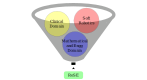
\includegraphics[width=\linewidth]{images/Ch1/fig2_funnel}} \quad
	\caption[Relationship between RoSE and different research domains.]{Relationship between RoSE and different research domains. \ac{RoSE} combines and integrates the concepts from four research domains: clinical, mathematical, engineering, and soft robotics}\label{fig2_funnel}
\end{figure}

\subsection{Motivation 2}

Conventional methods for discovering the partial \ac{DE}
of a system are rooted in laws of physics, conservation laws,
and phenomenological behavior. In any case, there remain numerous
complex systems like \ac{RoSE} that have escaped quantitative investigative
depictions or even characterization of an appropriate selection of
variables.
Currently, \ac{RoSE} does not have any dynamic equation to describe its
actuation principles or its physics. Finding out its governing \ac{DE} will not only help in better understanding its physics,
but it will also contribute to design a better adaptive close loop control
strategy for the robot, which can control the bolus transit behavior
by receiving feedback from the displacement sensors located on the
surface of the conduit. Instead of designing a black-box model of the
robot for control, a grey box model can be implemented, if some of
the dynamics of the robot are known.
In addition, a large number of different types of experiments with
manometry, videofluoroscopy, articulography, and motion capture
have already been performed on the robot resulting in the collection of
an extensive amount of datasets. Discovering the \ac{DE} from the collected datasets will give relevance to it as well as
meaning to the accomplished experiments.

\section{Aim and Objectives}

This study has two key aims. Firstly, the aim is to validate the application of \ac{RoSE} in performing a wide-ranging assessment of stent-related measurements and behavior for substantial equivalence. Secondly, the aim is to actuate the \ac{RoSE} conduit with pre-defined peristaltic wave trajectories by data-driven ML-based modeling and control. While the former aim, addresses the question of usability of \ac{RoSE} in the area of endoprosthetic stent testing, the later offers a novel approach to model and control \ac{RoSE} for understanding its underlying dynamics.  Objectives 1, 2, and 3, 4 will contribute to the fulfillment of the first and second aims, respectively.  With the accomplishment of the primary aim, \ac{RoSE} can emerge as a powerful in vitro platform for the endoscopic industries and clinicians to test their new stent designs in terms of migration and the occurrence of any kind of dysfunctionality during and after the stent implantation. The completion of the second aim will enhance this capability of \ac{RoSE} further. 

\subsection{Objective 1: RoSE Capability in Investigating Stent Radial Force and Migration.}

The objective assesses the effect of stent \ac{RF} on the migration of stents in the \ac{RoSE} conduit, which occurs due to repeated peristaltic contractions. The presented results can validate \ac{RoSE} as a novel platform to assess various stent behaviors, which can help the researchers and the endoscopists to elucidate the patency of the stents in the occurrence of unfavorable events, during and after the stent implantation. The objective was achieved by completing the following subtasks (\autoref{fig3_Obj1}):

\begin{figure}[bth]
	\myfloatalign
	{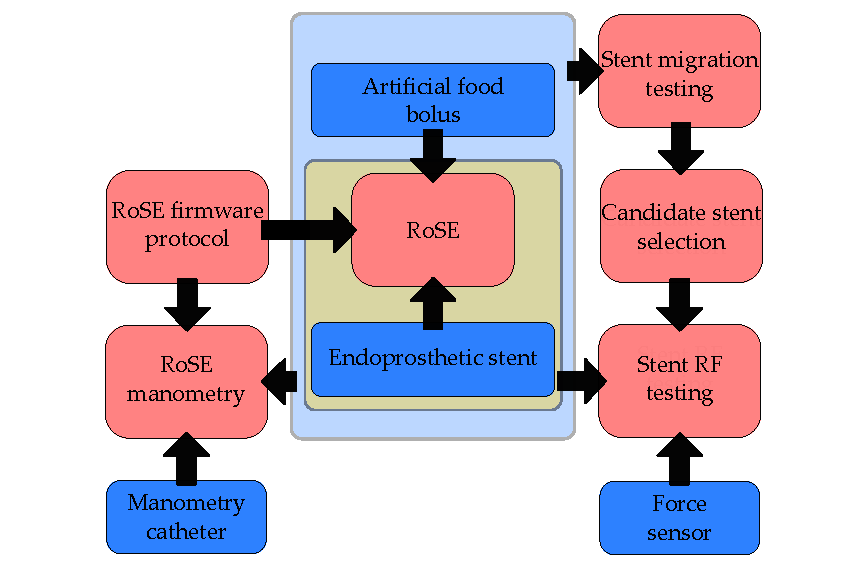
\includegraphics[width=\linewidth]{images/Ch1/fig3_Obj1}} \quad
	\caption[Sequence of the conducted subtasks to achieve objective 1 and 2.]{Sequence of the conducted subtasks to achieve objective 1 and 2.}\label{fig3_Obj1}
\end{figure}

\begin{itemize}
	\item Literature review
	
	Validating the capability of \ac{RoSE} in the area of stent testing requires reviewing relevant literature which underlines the major stent designing parameters and their effect on the stent performance. State of the art incorporating various topics on clinical studies on stent implantation, mathematical stent modeling, stent \ac{FEM}, and stent in vitro testing are studied for the attainment of the objective.  Besides, a thorough literature review on swallowing, \ac{EC}, and dysphagia is also conducted. 
	
	\item Development of RoSE firmware protocol
	
	Custom firmware modules, written in Python 3.7, are developed on Raspberry Pi 3B+ to assert the robot, with independent, continuously variable, pressure input. The \ac{RoSE} firmware protocol is divided into two significant sub-modules for stent \ac{RF}, and migration and bolus swallow efficacy testing. While, the first sub-module deals with simultaneous inflation and deflation of the \ac{RoSE} conduit, the second one generates peristaltic waves in \ac{RoSE}.
	
	\item Designing stent deployment framework
	
	A deployment framework following the endoscopists approach to deploying stents in the human esophagus was developed and employed throughout this study. 
	
	\item Artificial food bolus formulation
	
	Food boluses of varying consistencies were prepared in the laboratory using a commercial food thickener, specially formulated for dysphagia patients. The consistencies were quantified by evaluating the viscosity using a viscometer.
	
	\item Stent migration testing
	
	Five commercial, covered \ac{SEMS}s having distinct structures, cover materials, and cover material patterns, and similar dimensions were initially tested for stent migration in \ac{RoSE} with and without food bolus. Based on the maximum and minimum recorded migration,  candidate stents were selected for further measurement and analysis of different stent-related parameters.
	
	\item Force Sensor testing for RF measurement
	
	\item Stent RF testing
	
	By contracting and expanding the \ac{RoSE} conduit, stent \ac{RF} testing was performed. The testing protocol consists of repeatedly measuring the \ac{RF} applied by the stent on the conduit wall during its loading and unloading to evaluate its migration behavior. 
\end{itemize}

\subsection{Objective 2: RoSE In Vitro Platform for Studying the Impact of Stent Implantation on Bolus Swallow Efficacy.}

The objective is to examine the impact of the stent deployment on the \ac{RoSE} bolus swallow efficacy. Besides, it also includes analyzing the effect of stent dysfunctionality on bolus transport, and hence, swallow efficacy. \ac{RoSE} manometry investigation presents evidence that extends the knowledge of swallow efficacy after stent implantation during dysphagia (\autoref{fig3_Obj1}). 

\begin{itemize}
	\item Manometry setup and calibration
	
	A manometry setup consisting of a catheter (long flexible tube) and a data acquisition system was calibrated before installing the catheter into the \ac{RoSE} conduit due to the inaccessibility and unavailability of suitable instruments for in situ calibration. The catheter was positioned akin to the clinical in vivo observations.  
	
	\item RoSE manometry testing
	
	The methodology of \ac{RoSE} manometry testing can be distributed into two steps. In the first step, experiments and investigation for a regular stent operation were conducted, then in the second step, study for stent dysfunctionality was carried out. The investigation used both qualitative and quantitative analysis in order to gain insights into the effect of \ac{RoSE} swallow efficacy with implantation of stents. 
\end{itemize}
\subsection{Objective 3: Sparse Data-Driven Discovery of RoSE Dynamic Differential Equations}

The third objective is to discover the underlying dynamic \ac{DE} of \ac{RoSE}
by applying data-driven ML techniques. The \ac{DE} captures the \ac{RoSE}
peristaltic conduit deformation with respect to the applied pressure at
any instant of time. In contrast to previous \ac{RoSE} models, the \ac{DE} model
is dynamical in nature and solely depends on the captured data. The
model enhances the understanding of the kinematic and dynamic
features of \ac{RoSE}. The following tasks were undertaken to achieve this
objective (\autoref{fig4_Obj3}):

\begin{figure}[bth]
	\myfloatalign
	{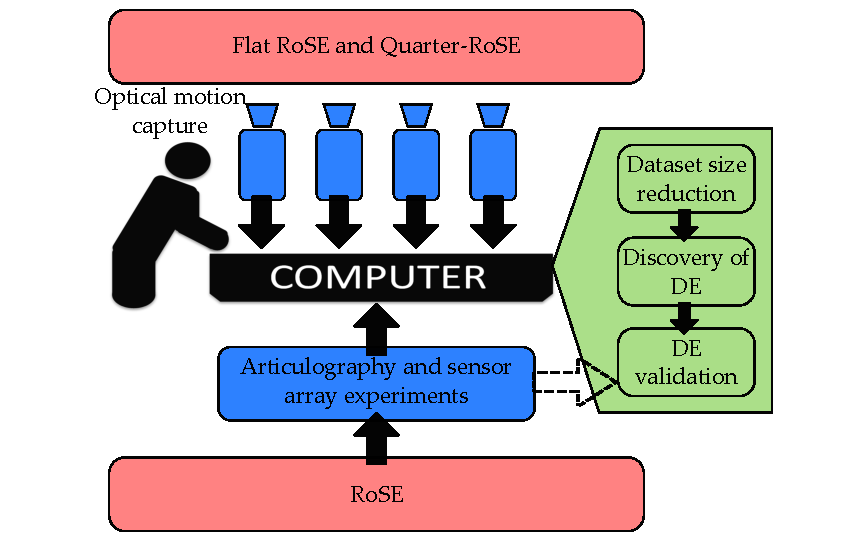
\includegraphics[width=\linewidth]{images/Ch1/fig4_Obj3}} \quad
	\caption[Sequence of the conducted subtasks to achieve objective 3.]{Sequence of the conducted subtasks to achieve objective 3.}\label{fig4_Obj3}
\end{figure}

\begin{itemize}
	\item Literature review
	
	Literature from the areas of \ac{ROM}, ML,
	and soft robotics was reviewed to analyze the existing modeling
	strategies. Various ML techniques were explored, along with their
	working principle and limitations. Besides, a thorough literature
	review on swallowing and dysphagia were also conducted.
	
	\item Design of Quarter-RoSE
	
	\ac{RoSE} has limited visibility inside its conduit, which challenges the
	collection of the experimental data needed for the \ac{DE} discovery.
	To address this issue, a \ac{QRoSE}
	was developed to observe and model the occlusive motion of the
	conduit of \ac{RoSE}.
	
	\item Optical motion capture
	
	To capture \ac{QRoSE} conduit deformation data, a column of retroreflective
	markers were placed on the conduit. By using the Vicon
	optical motion capture system, time-series datasets were collected
	by tracking the movement of the markers.
	
	\item Dataset size reduction
	
	To reduce the computational complexity, \ac{ROM} techniques were
	applied to the size of the collected dataset.
	
	\item Discovery of RoSE DE
	
	A data-driven ML technique which promotes sparsity was applied
	on the reduced dataset to discover the \ac{DE} of \ac{RoSE}.
	
	\item Validation of the DE
	
	The conduit deformation calculated from the discovered \ac{DE} was
	validated by collecting data from articulography and stretchable
	displacement sensor array experiments.
\end{itemize}

\subsection{Objective 4: Design of Sparse Model-Based Predictive Controller}

\section{Scope}

The first part of the research was about validating the applicability of \ac{RoSE} in the area of stent design and testing that can help the researchers and the endoscopists to elucidate the patency of the stents in the occurrence of unfavorable events, during and after the stent implantation. To clarify the extent, the study remains within the following research criteria. 

\begin{itemize}
	
	\item Even though \ac{RoSE} mimics the esophagus in various physiological ways but its conduit still lacks artificial strictures. Thus, all the multiple stent testings were carried out in normal swallowing conditions of RoSE.  
	
	\item The investigation of the stent testing has not considered the distribution of different muscle fiber regions because the entire \ac{RoSE} conduit is made up of the same silicone rubber material (Ecoflex 0030, Smooth-on, USA).
	
	\item The study is strictly limited to proving the usability of \ac{RoSE} in stent testing. It does not focus on the various design aspects of the stents that were used for conducting this research.

\end{itemize}

The second part of the research was about finding novelty in the area of soft robotics by implementing \ac{ML}, and optimization techniques to model and control \ac{RoSE} under different bolus transit behavior. Therefore, it abides the following research criteria:

\begin{itemize}
	\item  The derivation of the \ac{DE} of \ac{RoSE} has not considered the variation in properties of the material used to design the robot. The assumption only discusses the current state of the material and neglect any change in its qualitative or quantitative characteristics over time and varying environmental conditions like pressure and temperature.
	
	\item Any given marker on the surface of the robot moves along pre-defined coordinates of the x, y, and z-axis. For this research, movement along the y and z-axis are considered.
	
	\item All the sensors implemented in this research are off-the-shelf since the performance of the earlier designed and fabricated sensors are not up to the desired level.   

\end{itemize}

\section{Research Contributions}


Investigating stent \ac{RF} has been a continuing concern within the clinicians and the scientific community. It has been challenging to fully predict the clinical outcome of a stent based on its \ac{RF}. However, the presented results show that \ac{RoSE} can provide a novel platform to evaluate the substantial equivalence of esophageal stents of different characteristics. Besides, the results can provide the researchers with a deep insight into the patency of the stents and bolus swallow efficacy in the esophagus after stent implantation. The findings can make an essential contribution to the field of stent designing and testing. 

The results comparing the efficiency of the stents could aid the endoscopists in the selection of a suitable stent for an individual patient, which is otherwise guided solely by their experience and availability of the stents. The results will also aid in the optimization of future stent designs to improve the behavior of the stent during deployment and to mitigate migration. 

The analysis of the bolus pressure signatures with stenting in \ac{RoSE} has extended the knowledge of swallow efficacy after stent implantation during dysphagia. The presented in vitro study adds to the growing body of research that considered esophageal peristalsis for stent-related measurements. To the extent of our knowledge, no prior research has done endoscopic manometry in the presence of stents.  Additionally, the study has been one of the first attempts to examine parametric studies correlating the effect of stent implantation, and dysfunctionality on swallow efficacy. 

Soft robotic techniques provide compliance and unique shapes
to robots. In contrast to the rigid-bodied robots, soft robots have an advantage of infinite degrees of freedom, which allows them to move freely and mimic various movement patterns of humans. However, when it comes to modeling and control, the advantage becomes a disadvantage because all the parts of the robot continuously interact and inspire each other.  This study makes several noteworthy contributions to the
area of soft robotics modeling. To the best of our knowledge, this is the first time that ML has been applied to identify a structural and
parametric dynamical model of \ac{RoSE}. The methods revealed
the underlying dynamics of the soft-bodied \ac{RoSE} in the form of
\ac{DE} model. In contrast to the earlier models of \ac{RoSE}, the
the model presented in this research is dynamical. Since ML solely depends on the captured data, the discussed methodology is not robot specific and does not depend upon the actuation system and morphology of the robot. The method undertaken in this study is general, while \ac{RoSE} is a case study. It can be extended to any soft-robotic system, provided an input-output dataset can be generated. The \ac{DE} discovered in this
study also explicitly define the nonlinear behavior of the robot.
The analysis of the \ac{DE} has extended our knowledge about the
deformation of the \ac{RoSE} conduit. 
%*****************************************
%*****************************************
%*****************************************
%*****************************************
%*****************************************
